\section{Taxonomy similarity}

In this section, we propose a new similarity to quantify the different kinds of relatedness of terms based on a taxonomy tree and propose the corresponding efficient string join algorithms.


\subsection{Similarity with taxonomy trees}


The key to an efficient, uniform mechanism for set-at-a-time
(join-based) matching of query graph patterns is a positional
representation of occurrences of  elements and in the taxonomy database (see, e.g., [6, 7, 27]),
which extends the classic inverted index data structure in information retrieval [22]. We borrow the labeling scheme from XML databases and use the prefix based labels. Structural relationships between tree nodes whose positions
are recorded in this fashion can be determined easily for IS-A relationships.

\smallskip
\smallskip

\begin{definition}[Taxonomy Similarity]
Given two taxonomy tree nodes $n_1$ and $n_2$ with their prefix labels $L(n_1)$ and $L(n_2)$,  the similarity TS($n_1$,$n_2$) is the longest common prefix of  $n_1$ and $n_2$ over the length of the shorter path between $n_1$ and $n_2$, that is,  TS($n_1$,$n_2$,$\mathcal{T}$) = $\frac{|LCP(L(n_1),L(n_2))|}{min(|L(n_1)|,|L(n_2)|)}$. \end{definition}

\smallskip
\smallskip


\begin{example}
Consider Figure \ref{fig:taxonomyexample}, the similarity between ``\textsf{Seoul}'' (3.1.1.1) and ``\textsf{Suwon}'' (3.1.1.2) is $\frac{3}{4}$= 0.75 (as both countries are in South Korea.), and the the similarity between ``\textsf{Seoul}''  (3.1.1.1) and ``\textsf{Shenzhen}'' (3.2.1.1) is only $\frac{1}{4}$= 0.25 (as two countries are in Asia).
\end{example}

\smallskip
\smallskip

\begin{lem} Given two nodes $n_1$ and $n_2$ in a taxonomy tree, if there are the ancestor-descendant relation between $n_1$ and $n_2$, then $TS(n_1,n_2)$ = 1.
\end{lem}

\begin{proof} Since $n_1$ and $n_2$ have the ancestor-descendant relation, without loss the generality, assume that $n_1$ is the ancestor of $n_2$, then $|LCP(n_1,n_2)|$ = $|n_1|$ and min($|n_1|,|n_2|$) = $|n_1|$. Therefore, TS($n_1,n_2$) = 1.
\end{proof}


\subsection{Join algorithms}


We would formulate the string similarity join problem and develop the corresponding algorithms. Given two collections of strings $S$ and $T$, a taxonomy tree
$\mathcal{T}$, and a similarity threshold $\theta$, a \textit{string
  similarity join} finds all string pairs $(s, t) \in S \times T$,
such that $TS(s,t,\mathcal{T})$ $>$ $\theta$, where \textit{TS} is
 the taxonomy similarity functions defined above.



Given two collections of strings $S$ and $T$, the baseline join algorithm is the nested-loop join. All string pairs are accessed to determine the IS-A relationships. But this algorithm is obviously not efficient. Therefore, we propose an efficient algorithm.



\begin{figure}[t]
\centering
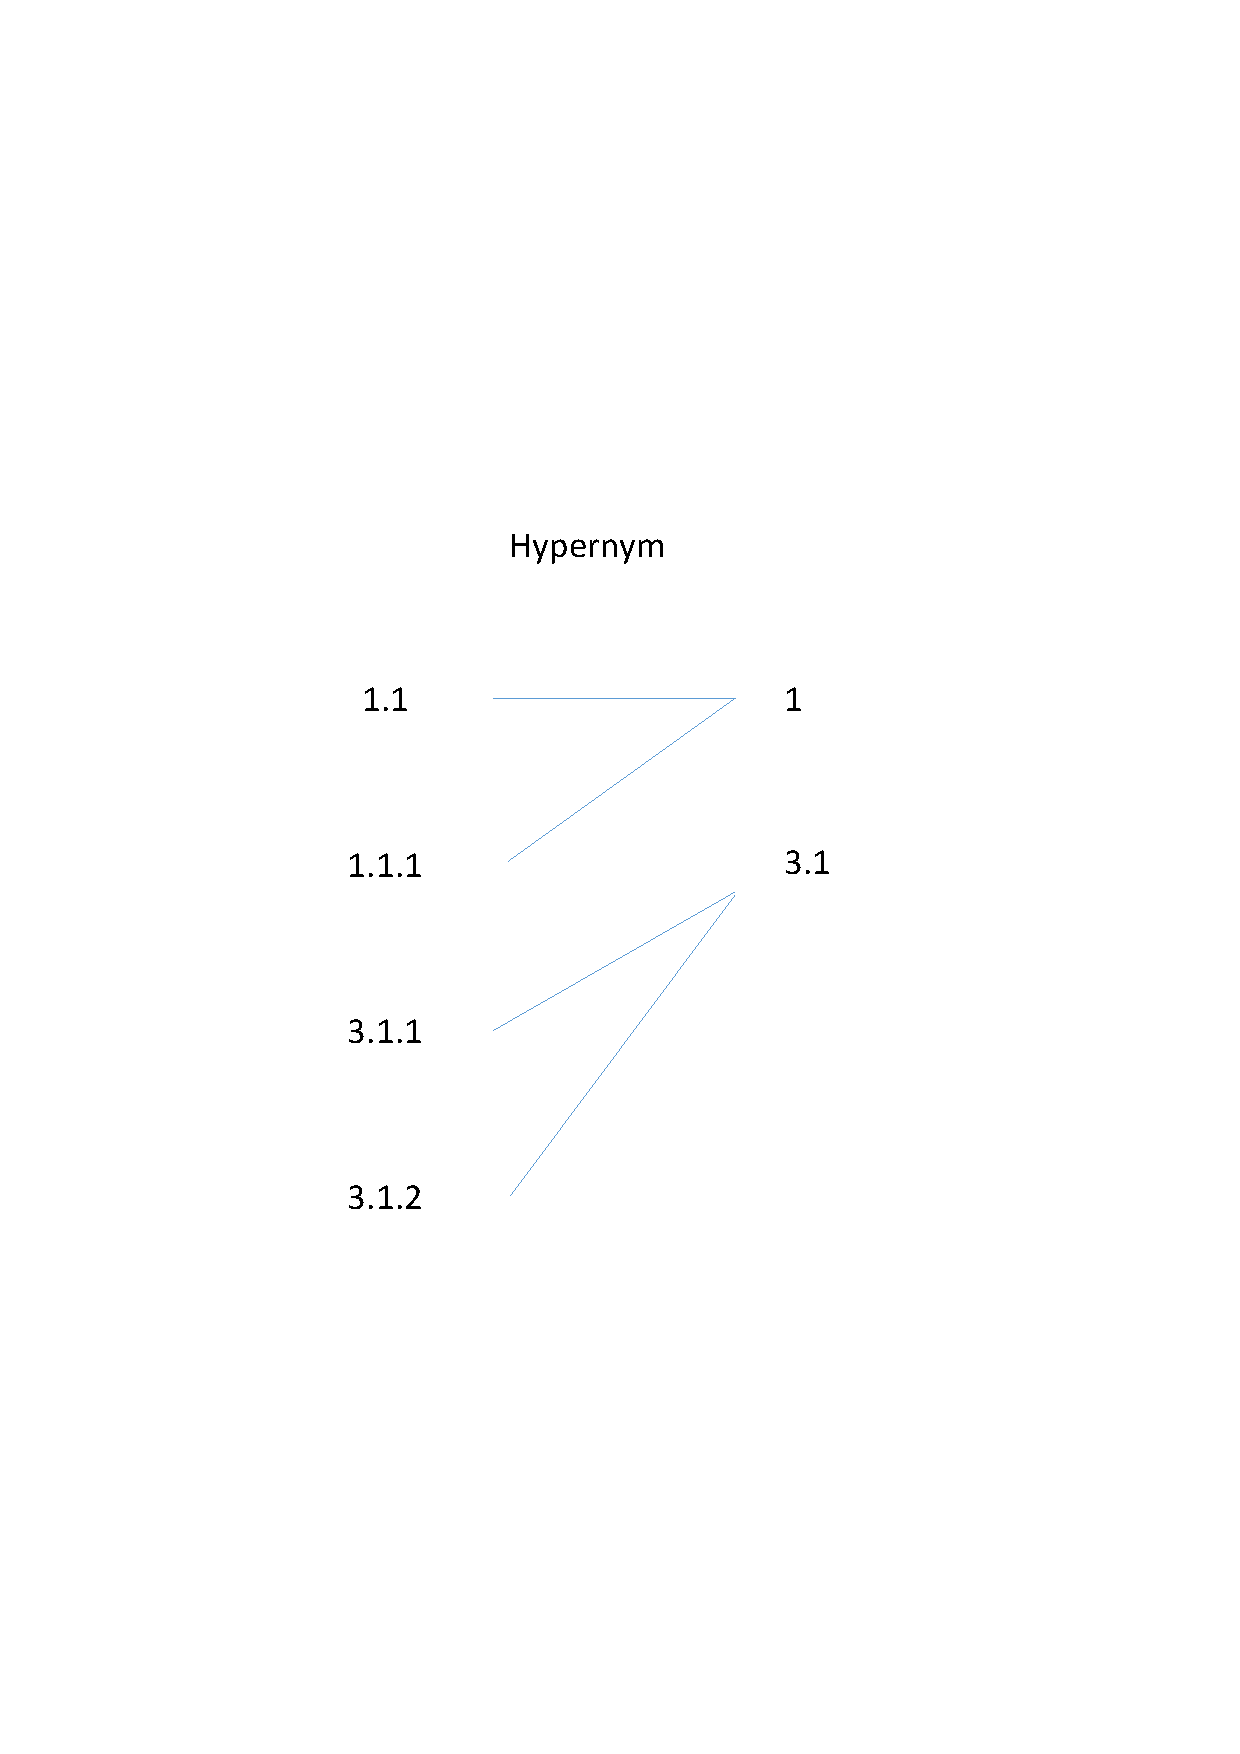
\includegraphics[scale=0.4]{figures/labeljoins}
 \caption{Join inverted lists}
\label{fig:invertedlist}
\end{figure}


%\begin{algorithm}
%{\bf Input}: two strings $s_1$ and $s_2$ \\
%{\bf Output}: four relationships: R=\{Hype, Hypo, Equa and Non\}
%\begin{compactenum}[(1)]
%\item {\bf If} ($s_1 = s_2$ )  {\bf return} Equa;
%\item {\bf If} ($|LCD(s_1)| >$ 1 AND $|LCD(s_2)| >$ 1 )  {\bf return} None;
%\item {\bf Else} {\bf if} ($|LCD(s_1)| =$ 1 AND $|LCD(s_2)| >$ 1 )
%\item \verb"  " {\bf If}  $\forall t \in LCD(s_1)$, $t$ is a hypernym of $LCD(s_2)$
%\item \verb"    " {\bf return} Hype {\bf else} {\bf return} None;
%\item {\bf Else} {\bf if} ($|LCD(s_2)| =$ 1 AND $|LCD(s_1)| >$ 1 )
%\item \verb"  " {\bf If}  $\forall t \in LCD(s_2)$, $t$ is a hypernym of $LCD(s_1)$
%\item  \verb"    " {\bf return} Hypo {\bf else} {\bf return} None;
%\item {\bf Else} /\ *  $|LCD(s_1)| = |LCD(s_2)| = $ 1 */\
%\item  \verb"  " {\bf If}  $LCD(s_1)$ is a hypernym of $LCD(s_2)$  {\bf return} Hype
%\item   \verb"  " {\bf Else if}  $LCD(s_1)$ is a hyponym of $LCD(s_2)$  {\bf return} Hypo
%\item   \verb"  " {\bf Else return} none
%\end{compactenum}
%\caption{Determine the relationship between two strings}
%\label{alg:measure}
%\end{algorithm}





\begin{algorithm}
{\bf Input}: two sets of strings $S$ and $T$, a taxonomy $\mathcal{T}$, a threshold $\theta$ \\
{\bf Output}: string pairs $(s_1,s_2) \in S_1 \times S_2$, s.t. $TS(s_1, s_2) > \theta$
\begin{compactenum}[(1)]
\item Let $T_s$ and $T_t$ denote two prefix trees for $S$ and $T$ respectively.
\item {\bf FOR} EACH leaf node $n$ in $T_s$ DO
\item ~~~ $R_1$ = findTS(n,$\mathcal{T}$,$\theta$);
\item {\bf FOR} EACH join pair ($t_1,t_2$)$\in R_1$
\item  Add $t_1.List \times t_2.List$ to R;
\item RETURN $R$
\end{compactenum}
\caption{String joins with taxonomy}
\label{alg:exactjoin}
\end{algorithm}


\begin{algorithm}
{\bf Input}: A node n in $T_s$ and prefix $P$ of n in $T_s$ and a threshold $\theta$ \\
{\bf Output}:  pairs $R$ = \{$(n,m) \in L_1 \times L_2$ s.t. $TS(n,m) > \theta$\}
\begin{compactenum}[(1)]
\item FOR EACH i=1 to $|n|$
\item ~~~ $l$ = $\lceil \theta \cdot i \rceil$
\item ~~~ $p$ = $prefix(n,l)$
\item ~~~ IF $i < |n|$ AND $p \notin P$ THEN
\item ~~~~~~~ Add all nodes in $T_t$ with the length $i$ and the prefix $p$ to R;
\item ~~~ ELSE   
\item ~~~  ~~~  Add all nodes in $T_t$ with the prefix $p$ to R;
\end{compactenum}
\caption{findTS(n,T,$\theta$)}
\label{alg:treejoin}
\end{algorithm}


Associated with a collection $T$ there is a list $L_T$. This list contain the positional representation of the taxonomy tree nodes that match strings in the $T$. The nodes in the list are sorted by the lexicographical order. The operation over lists are: Eof, advance, next.

In the findTS procedure, prefix(n,l) means to return the length-$l$-prefix of node $n$. For example, suppose $n$= 1.5.1.1,  prefix(n,3)=``1.5.1''.  

\smallskip
\smallskip

\begin{example}
Consider the node Seoul  (3.1.1.1). Then $|n|$=4, 
\end{example}

\smallskip
\smallskip


\begin{theorem}  Algorithm \ref{alg:exactjoin} is an optimal algorithm. The computing cost is linear to the sum of the size of the input and output. That is, each output result contribute to the final answer.
\end{theorem}




